\capitulo{3}{Conceptos teóricos}

\section{Aprendizaje automático}

 En inglés \emph{machine learning}, es un campo de la inteligencia artificial cuyo objetivo es desarrollar técnicas y algoritmos que permitan a las máquinas aprender, por si mismos, a través de la experiencia. Sus principales usos del aprendizaje automático son la detección de patrones, reconocimiento de lenguajes, vehículos autónomos, vídeojuegos, y muchas otras áreas. 
    
 Para desarrollar el aprendizaje se usa un modelo matemático basado en datos de entrenamiento para así realizar predicciones o decisiones sin ser programados para hacer estas tareas~\cite{ Zhang2020}.
    
 Dependiendo del modelo de datos que tengan los algoritmos se pueden agrupar en:
 
 \begin{itemize}
 
  \item \textbf{Aprendizaje supervisado:} establece correspondencias entre los datos de entrada y los de las salidas deseadas. Parte de ejemplos resueltos para luego resolver problemas semejantes.
  
  \item \textbf{Aprendizaje no supervisado:} solo usa los datos como entrada sin saber la clase a la que pertenecen dichos datos. Infiere tanto la forma de las agrupaciones de los datos, como la clase a la que pertenecen.
  
  \item \textbf{Aprendizaje semi-supervisado:} es una mezcla entre el aprendizaje supervisado y el no supervisado, hay una pequeña parte de los datos que se saben a qué clase pertenecen y el resto no.
  
  \item \textbf{Aprendizaje por refuerzo:} el algoritmo aprende observando su entorno, los datos de entrada se basan en la retroalimentación de sus acciones, cuando actúan de forma correcta son recompensados, si no, son penalizados.
  
  \item \textbf{Aprendizaje por transferencia:} consiste en utilizar un modelo preentrenado para una tarea y reutilizarlo para resolver una tarea distinta tras algunos pequeños ajustes iniciales. La idea es que las características de bajo nivel que haya aprendido el modelo puedan reutilizarse, aunque tenga que cambiarse como se combina estas para resolver la nueva tarea. 
  
 \end{itemize}

\section{Restauración de vídeos mediante inteligencia artificial}
 La restauración tanto de vídeos como de imágenes actualmente está avanzando exponencialmente demostrando resultados sorprendentes respecto de los obtenidos hace escasamente unos pocos años. La mayoría de técnicas que surgen actualmente se basan en un aprendizaje supervisado usando un par de imágenes una \emph{GROUND-TRUTH}, la imagen ideal que se tiene por referencia y otra \emph{LOW-RESOLUTION}, que es la misma imagen en baja calidad generada por un modelo de degradación como puede ser un sub-muestreo de tipo lineal o vecino más cercano.
 Estas técnicas no acaban de adaptarse completamente a las situaciones reales, ya que estas presentan una complejidad mucho mas pronunciada que la generada por el proceso de submuestreo ~\cite{9359916}.

 Así mismo las técnicas de restauración deben ser capaces de conseguir los resultados intentando ser lo más eficientes en el tiempo empleado y en los recursos consumidos, memoria y energía, siendo ejecutados en hardware común.
 
 La principal diferencia entre la restauración de vídeos e imágenes radica en que los vídeos suponen una complejidad extra, el aspecto temporal, teniendo en cuenta que las imágenes que lo componen están relacionadas entre sí. ~\cite{8746778}.

 Los aspectos en los que se centran los métodos de restauración de vídeos son los siguientes:
 \begin{itemize}

    \item \textbf{Reducción de ruido:} o \emph{denoising} en inglés, consiste en la eliminación de información que corrompe la señal de vídeo debido a problemas en el canal o proceso de adquisición y/o de transmisión.
    \imagen{ruido}{Ruido generado por mala iluminación (Imagen adquirida por el autor)}
        
    \item \textbf{Eliminación del emborronamiento:} proceso de eliminar aspectos borrosos o distorsionados de las imágenes, que se puede deber al movimiento del objeto a capturar o al movimiento en el momento de la captura del dispositivo de grabación. También puede generarse cuando no hay un correcto enfoque de la lente.
    
    \item \textbf{Eliminación de niebla:} mejorar la calidad de una imagen que se encuentre degradada por causas atmosféricas o por partículas en suspensión en el aire que impiden el reconocimiento parcial de la imagen. ~\cite{inproceedings}
    \imagen{dehaze}{Ejemplo de dehazing (Imagen adquirida por el autor).}

    \item \textbf{Super resolución:} técnicas y algoritmos que parten de una imagen con baja resolución y la transforman en una de mayor resolución, obteniendo un número mayor de píxeles donde se recupera la información de los detalles. Existen múltiples clasificaciones y metodos de super resolución, la más típica son:
        \begin{itemize}
           \item \textbf{Multiframe:} técnica de procesado de imágenes que a partir de un conjunto de imágenes, correspondientes a posiciones espaciales diferentes de la cámara genera una sola imagen en alta resolución. El aspecto temporal influye mucho a la hora del procesado de imágenes~\cite{7919264}.
           
            \item \textbf{Single frame:} técnica de procesado de imágenes que a partir de una sola imagen en baja resolución produce una imagen en alta resolución. No se suele usar en la super resolución de vídeos ya que los vídeos suelen presentar mayor complejidad para su super resolución, lo que no quita que haya muchas opciones para elegir. 
        \end{itemize}
        
     \item \textbf{Compresión:} algunos formatos de imagen tienen una compresión por defecto para reducir el tamaño que ocupan y por lo tanto  pueden perder detalles, por eso se usan métodos para recuperar las pérdidas de información ~\cite{Wang_2016_CVPR}.
     
 \end{itemize}
 
\section{Reconocimiento de acciones}
 El reconocimiento de acciones humanas tiene múltiples aplicaciones, pero sobre todo en vigilancia, análisis de contenido e interacciones entre humanos y ordenadores. El reconocimiento debe ser automático tanto de acciones simples como complejas. Una acción es una secuencia de movimientos que puede  comprender varias partes del cuerpo humano.
 
 \subsection{Tipos de acciones}
  Clasificación según el tipo de acción:
 \begin{itemize}
 
 \item \textbf {Acciones simples:} Los llamados gestos o las acciones que no pueden reducirse a otras más sencillas. Negar con la cabeza, saludar, levantar un pie, son ejemplos de este tipo de acciones.   
 
 \item \textbf {Acciones complejas:} Son una combinación de acciones simples.  Andar, correr, dar un salto, entran es esta clasificación.
 
 \item \textbf {Interacciones:} Son las acciones que surgen de la interacción entre grupos reducidos de personas u objetos. Dos personas dándose la mano, o alguien tocando un instrumento.
 
 \item \textbf {Actividades de grupo:} Las acciones que envuelven a un gran número de personas, como un desfile o una calle concurrida.

  \end{itemize}
 Los dos primeros grupos de acciones, simples y complejas son las que han sido más estudiadas y mejores resultados ofrecen. No obstante, recientemente, hay más esfuerzos que se centran en las interacciones y grupos.
 
 En el contexto de la inteligencia artificial, el objetivo consiste en identificar las acciones de un vídeo con otras  previamente identificadas y así asignarle una etiqueta a cada tipo de acción.  El proceso simplificado consiste en la detección de la persona o partes del cuerpo, el seguimiento de las identificaciones  y por último la asignación del tipo de acción, comparando la información obtenida, con sus conocimientos obtenidos mediante el entrenamiento.
 
  \subsection{Clasificación de algoritmos de reconocimiento de acciones}
  
  A la hora de  seleccionar el algoritmo para la clasificación de los gestos o acciones existen una gran variedad de opciones. A continuación se exponen de forma resumida las consideradas más importantes.
  \begin{figure}[!ht]
		\centering
		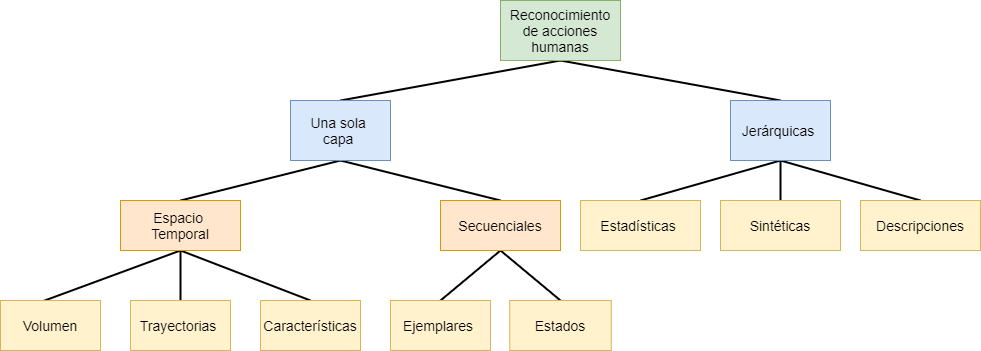
\includegraphics[width=1.1\textwidth]{recoAcciones2}
		\caption{Tipos de algoritmos de reconocimiento de acciones~\cite{article}}\label{1}
	\end{figure}
	\FloatBarrier

         \begin{itemize}
         
            \item \textbf {Una sola capa:} Las acciones se reconocen directamente del vídeo, sin diferenciar en acciones más simples.
            
             \begin{itemize}
             
                \item \textbf {Espacio temporal:} Se basan tanto en la información espacial (imagen 2D), como en la información proporcionada por la variable temporal ($t$), analizando sus interdependencias. Se basan en fijar  unos puntos y estudian su trayectoria en el espacio.
                
                \item \textbf {Secuenciales:} Están diseñados para captar las relaciones temporales de las observaciones, las acciones humanas se integran como una secuencia de observaciones. Una observación se asocia con características extraídas de un conjunto.
                
             \end{itemize}
             
             \item \textbf {Jerárquicas:} Buscan momentos relevantes en las acciones más sencillas, una acción compleja se divide en varias más simples.
             
          \end{itemize}
  
